%%% intro on LHC 
%%% ATLAS and HGTD
%%% 

\chapter{Introduction}

\section{The LHC and the High Luminosity upgrade}

The Large Hadron Collider (LHC)is the largest particle accelerator in the world. Built between 1998 and 2008 by the European Organization for Nuclear Research (CERN, \textit{Conseil européen pour la Recherche nucléaire}) in collaboration with more than 100 countries. 
It achieved beam energies of more than 6.5 TeV and enabled many historic discoveries in particle physics.
Along the accelerator track there are four main experiments: ALICE, ATLAS, CMS, LHCb (Figure \ref{fig:LHC}). 

\begin{figure}[!h]
    \centering
    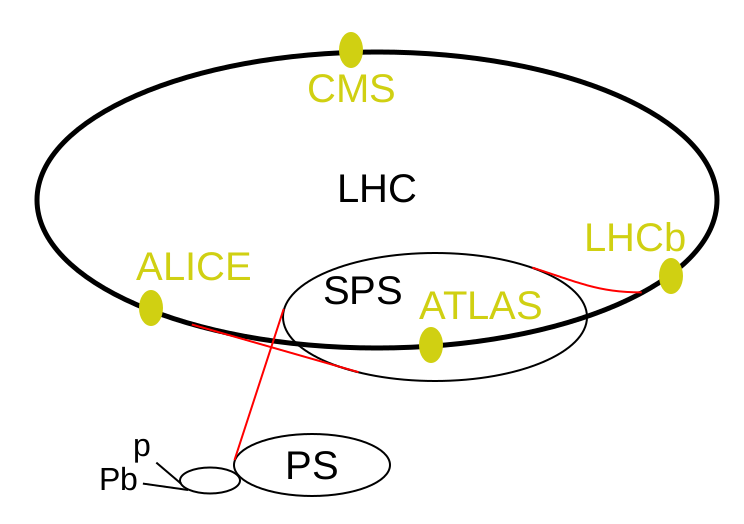
\includegraphics[width=.8\textwidth]{Images/intro/LHC.png}
    \caption{LHC scheme and the four main experiments. Each particle (typically proton or lead ion) is accelerated from the Proton Synchrotron into the Super Proton Synchrotron and finally into the Large Hadron Collider}
    \label{fig:LHC}
\end{figure}


The High-Luminosity phase of the Large Hadron Collider (HL-LHC), which should be operational in 2029 \cite{LS3_schedule_change}, aims to increase the integrated luminosity by a factor of 10 \cite{CERN-LHCC-2020-007}.
This will give great opportunities for new physics but it will also introduce a wide range of new challenges.

% this is already kinda talking about HGTD, maybe it's a good bridge to the next section: HGTD


\section{The ATLAS experiment and the HGTD}

ATLAS (\textbf{A} \textbf{T}oroidal \textbf{L}HC \textbf{A}pparatu\textbf{S}) is a general purpose detector built for probing \textit{p-p} and \textit{A-A} collisions (\textit{proton-proton} and \textit{heavy ion-heavy ion}, respectively). \marginpar{\flushleft can be improved}
The experiment's main components are: Inner Detector, Calorimeters and Muon Spectrometer \cite{Collaboration_The_ATLAS2008}.

\begin{figure}[!h]
    \centering
    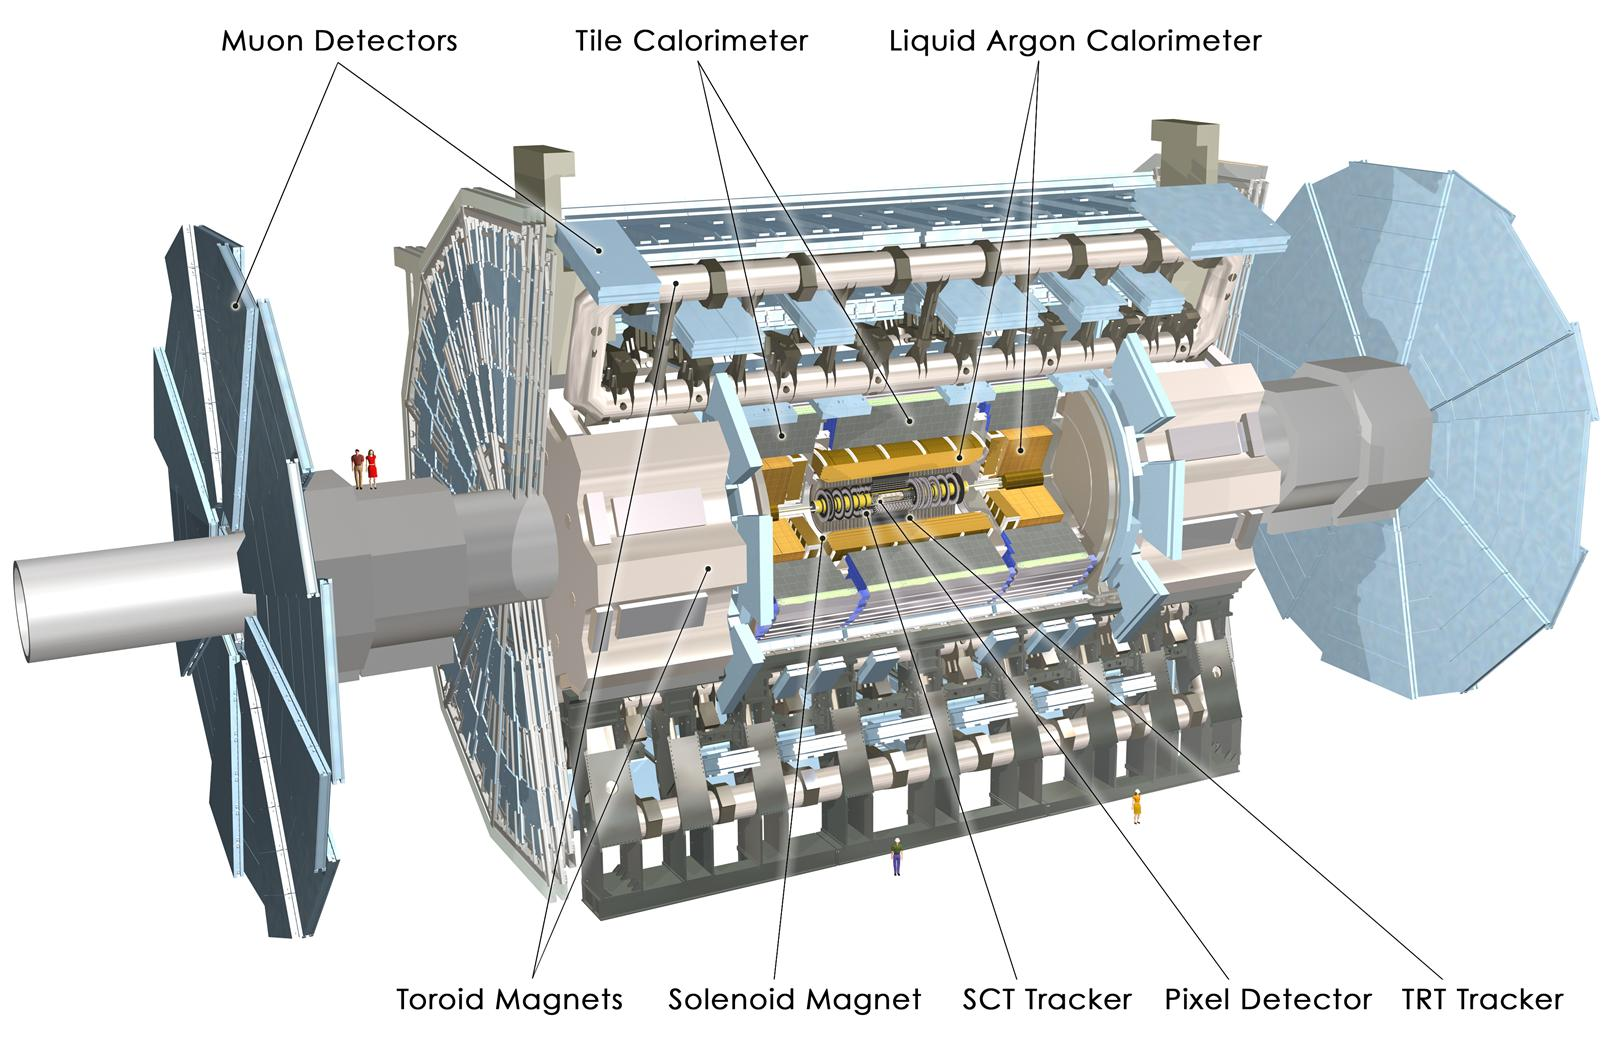
\includegraphics[width=\textwidth]{Images/intro/ATLAS_with_description.jpg}
    \caption{ATLAS experiment and its main components}
    \label{fig:ATLAS}
\end{figure}

A considerable challenge that will arise with the High Luminosity upgrade will be the increase of pile-up of events, i.e. collisions that will happen too close to each other to be individually resolved. 
A new way to mitigate this effect will be "\textit{to use high-precision timing information to distinguish between collisions occurring very close in space but well-separated in time}" \cite{CERN-LHCC-2020-007}. This is set to be accomplished by the High Granularity Time Detector (HGTD).

% picture of HGTD
\begin{figure}
    \centering
    \subfloat[Location]{
        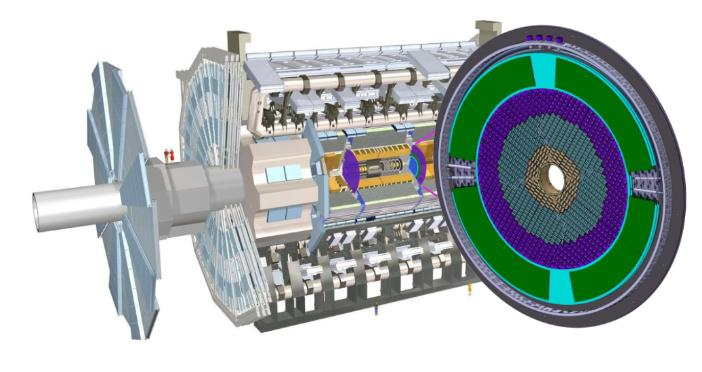
\includegraphics[width=.6\textwidth]{Images/intro/HGTD position and layout.jpg}
        \label{fig:HGTD_location}}
    \hfill
    \centering
    \subfloat[Schema]{
        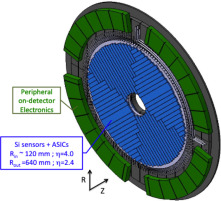
\includegraphics[width=.35\textwidth]{Images/intro/HGTD_schema.jpg}
        \label{fig:HGTD_schema}}
    \caption{Location and schema of the HGTD inside ATLAS}
\end{figure}

% eta=2.4 -> theta=10.367°      eta=4 -> theta=2.0986°
The detector will cover pseudrapidities between $2.4 < \eta < 4.0$ \footnote{the pseudorapity is $\eta=-\ln \tan(\theta/2)$ where $\theta$ is the polar angle from the $z$ axis, i.e. the beam direction.} (so an incident angle roughly between 2° and 10°), complementing the ITk (Inner Tracker) which has worse resolution in this forward region. The luminous region in the nominal scenario for Run 3 will see a Gaussian spread of approximately 50mm along the $z$ axis and a width of 175$\si{ps}$ in time (Figure \ref{fig:events_pileup}). HGTD will provide time information of charged particles with a time resolution of 30ps (up to 50ps at the end of life) which will greatly improve the reconstruction of the primary vertex of collision.


\begin{figure}[!hb]
    \centering
    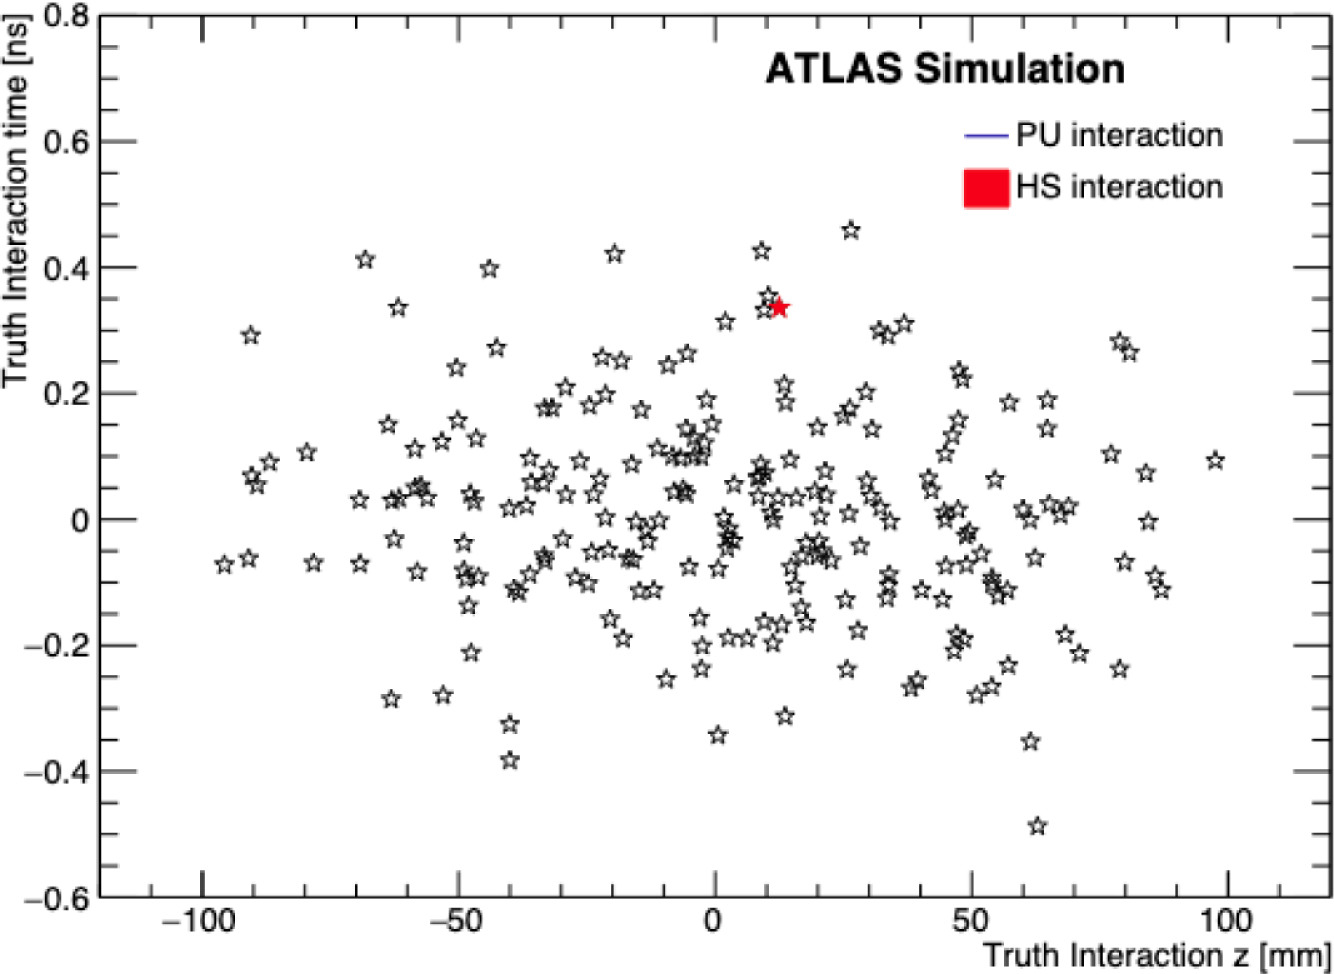
\includegraphics[width=.8\textwidth]{Images/intro/events_pileup_HL_LHC.jpg}
    \caption{Visualization of the pile-up of events inside ATLAS, using simulation data (PUT SOURCE AND MORE EXPLANATIONS (what is HS?))}
    \label{fig:events_pileup}
\end{figure}
